\documentclass[10pt]{article}
\usepackage[top=1in,bottom=1.1in,left=.8in,right=.8in]{geometry}
\usepackage[T1]{fontenc}
\usepackage[ansinew]{inputenc}
\usepackage{graphicx}
\usepackage{multirow}
\usepackage{url}

\renewcommand{\familydefault}{\sfdefault}

\begin{document}
%\maketitle

\hspace{-5mm}
\begin{minipage}{0.65\linewidth}
  \textbf{{\Large COMP 231\\
      Introduction to Computer Organization\\Lab 3}}
\end{minipage}
\begin{minipage}{0.35\linewidth}
  \includegraphics[scale=.3]{../../logos/rhodes-logo.jpg}
\end{minipage}

\vspace{.25in}

This lab will consist of a Quartus project folder, submitted as a
single ZIP file, via Canvas (\url{http://canvas.rhodes.edu/}).
{\bf You must submit a .zip file in the following format, otherwise
  you will lose points.} When you submit your project, rename the
project folder to <{\em name\_lab3}>, where the name is your Rhodes
email ID. Then, ZIP the folder up and upload it to Canvas. Do not
use any other compression/archiving format other than ZIP.

\section*{Overview}

In this lab, you will create a combinational and sequential logic
circuit that acts as a seven segment display (SSD) driver. The
circuit will display a single hexadecimal value on one of the LED SSD
devices on the DE2 board (see below for appropriate outputs for each hexadecimal number). The display consists of seven LED segments,
each of which are connected to a single pin:

\begin{center}

\includegraphics[scale=1.0]{sssd}
\end{center}

\section{Design}

You will design a circuit that takes a four-bit input value that
represents a single hexadecimal digit. Given the hexadecimal value,
the circuit will activate a set of seven output wires that will be
connected to the input pins of an SSD. For example, if the input is
{\tt 0000}, then the output of the function would activate lights
for pins 0--5 and not pin 6 of the SSD.

Write a truth table that completely describes the behavior of the
system (i.e.\ one column for each segment). Construct seven K-maps and
determine the AND-OR expressions for the minimum sum of products
(MSOP) equations for each of the seven outputs. You will submit this
work separately on paper (either in class or through Canvas).

The SSD is an ``active-low'' device, which means that a 0 value
illuminates the LED and a 1 turns it off. You can perform your design
normally and just add an inverter to the final result of the circuit
to get it to work correctly with active-low hardware.

\begin{center}
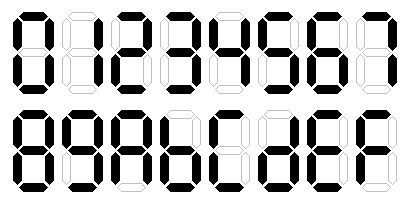
\includegraphics[scale=1.0]{hex7seg.png}
\end{center}

\section{Single SSD Circuit}

Using Quartus II, implement the system using a schematic design,
similar to that used in the last assignment. It is easiest to break
up the work into separate blocks for clarity and ease of
debugging. Start by creating a new schematic file for the top-level
project in the lab ({\tt lab3}).

Next, create a new schematic file for each output line of the
SSD (e.g. {\tt hex\_0}). Once you have implemented the circuit for an output line
(e.g. LED segment 0), save the file and select the ``{\it
  File$\rightarrow$Create/Update$\rightarrow$Create Symbol Files for
  Current File}'' menu item. This creates a circuit block that you can
use in other files. Each of these circuits should take four inputs and
produce a single output.

Once you have the seven building blocks created, make a new file, {\tt
  ssdd}, that represents the entire SSDD. Add each of the seven
sub-circuits to this module as you would any normal gate. Instead of
choosing a circuit from the Altera library, select each block from the
{\tt Project} menu. You may {\bf not} use any built-in SSD hardware or
anything more complicated than basic logic gates for your SSDD. Add
wires to connect the four input pins to each of the LED segment
drivers and each driver output to an output pin.

Lastly, back in the top-level schematic, {\tt lab3}, add the block for
your entire SSDD and connect the inputs to pins for SW[0..3] and
connect the output to pins for HEX0[0..6]. At this point you should
be able to input a 4-bit binary number using the switches and have the
correct value illuminate on the seven-segment display.

\section{Counter}

Create a new schematic file called {\tt counter}. In this file,
implement the four-bit counter as described in class and in the
book. For this block, you may use Altera library circuits for JK
flip-flops. They are under {\tt primitives $\rightarrow$ storage
  $\rightarrow$ jkff} in the gate chooser dialog. Do not attach any
wires to the {\tt PRN} or {\tt CLRN} inputs of the flip-flops.

Your counter circuit should take two inputs: a counter enable line,
and a clock signal. The counter should provide four output lines, one
for each bit of the counter. You do not need to provide a carry out.

\section{Tying It Together}

In your top-level file, remove {\tt SW[0..3]} input pins from the
SSD. Add an instance of your 4-bit counter circuit and connect the
output of the counter to the inputs of the SSSD. Map KEY[0] to the
clock signal and SW[0] to the clock enable. Using the keypad to
simulate the clock, ensure that the circuit counts from zero to {\tt
  F} on the SSD.

\section*{Submission}

When you have completed this entire exercise and have a functioning
program, submit your lab 3 project folder as specified above to Canvas.

\end{document}

